\documentclass[thesis=M,english,hidelinks]{inc/FITthesis}[2012/10/20]

\usepackage[utf8]{inputenc}

\usepackage{graphicx}
\usepackage{dirtree}
\usepackage{booktabs}
\usepackage{listings,xcolor}

% http://www.davehofmann.de/?p=153

\lstdefinelanguage{go} {
  morekeywords={
    import,
    if,
    while,
    for,
    type,
    interface,
    string
  },
  sensitive=true, % keywords are not case-sensitive
  morestring=[b]"
}
% Define Colors
\usepackage{color}
\definecolor{eclipseBlue}{RGB}{42,0.0,255}
\definecolor{eclipseGreen}{RGB}{63,127,95}
\definecolor{eclipsePurple}{RGB}{127,0,85}
 
% Set Language
\lstset{
  language={Go},
  basicstyle=\small\ttfamily, % Global Code Style
  captionpos=b, % Position of the Caption (t for top, b for bottom)
  columns=fixed, % make all characters equal width
  keepspaces=true, % does not ignore spaces to fit width, convert tabs to spaces
  showstringspaces=false, % lets spaces in strings appear as real spaces
  breaklines=true, % wrap lines if they don't fit
  frame=trbl, % draw a frame at the top, right, left and bottom of the listing
  framesep=4pt, % quarter circle size of the round corners
  numbers=left, % show line numbers at the left
  numberstyle=\tiny\ttfamily, % style of the line numbers
  commentstyle=\color{eclipseGreen}, % style of comments
  keywordstyle=\color{eclipsePurple}, % style of keywords
  stringstyle=\color{eclipseBlue}, % style of strings
}
%http://tex.stackexchange.com/questions/152829/how-can-i-highlight-yaml-code-in-a-pretty-way-with-listings
\newcommand\YAMLcolonstyle{\color{red}}
\newcommand\YAMLkeystyle{\color{blue}}
\newcommand\YAMLvaluestyle{\color{black}}

\lstdefinelanguage{yaml}
{
  keywords={true,false,null,y,n},
  keywordstyle=\color{darkgray}\bfseries,
  rulecolor=\color{black},
  basicstyle=\YAMLkeystyle,                                 % assuming a key comes first
  sensitive=false,
  comment=[l]{\#},
  morecomment=[s]{/*}{*/},
  numberstyle=\tiny\ttfamily\color{black},
  commentstyle=\color{purple}\ttfamily,
  stringstyle=\YAMLvaluestyle\ttfamily,
  moredelim=[l][\color{orange}]{\&},
  moredelim=[l][\color{magenta}]{*},
  moredelim=**[il][\YAMLcolonstyle{:}\YAMLvaluestyle]{:},   % switch to value style at :
  morestring=[b]',
  morestring=[b]",
  literate =    {---}{{\ProcessThreeDashes}}3
                {>}{{\textcolor{red}\textgreater}}1     
                {|}{{\textcolor{red}\textbar}}1 
                {\ -\ }{{\mdseries\ -\ }}3,
}

% http://www.davehofmann.de/?p=153

\lstdefinelanguage{dockerfile} {
  morekeywords={
    FROM,
    RUN
  },
  sensitive=true, % keywords are not case-sensitive
  morestring=[b]"
}
% Define Colors
\usepackage{color}
\definecolor{eclipseBlue}{RGB}{42,0.0,255}
\definecolor{eclipseGreen}{RGB}{63,127,95}
\definecolor{eclipsePurple}{RGB}{127,0,85}
 
% Set Language
\lstset{
  language={dockerfile},
  basicstyle=\small\ttfamily, % Global Code Style
  captionpos=b, % Position of the Caption (t for top, b for bottom)
  columns=fixed, % make all characters equal width
  keepspaces=true, % does not ignore spaces to fit width, convert tabs to spaces
  showstringspaces=false, % lets spaces in strings appear as real spaces
  breaklines=true, % wrap lines if they don't fit
  frame=trbl, % draw a frame at the top, right, left and bottom of the listing
  framesep=4pt, % quarter circle size of the round corners
  numbers=left, % show line numbers at the left
  numberstyle=\tiny\ttfamily, % style of the line numbers
  commentstyle=\color{eclipseGreen}, % style of comments
  keywordstyle=\color{eclipsePurple}, % style of keywords
  stringstyle=\color{eclipseBlue}, % style of strings
}

\department{Department of Software Engineering}
\title{Suitability analysis of Kubernetes for~Seznam.cz}
\authorGN{Ondřej}
\authorFN{Šejvl}
\author{Ondřej Šejvl}
\authorWithDegrees{Bc. Ondřej Šejvl}
\supervisor{Ing. Jan Baier}

\acknowledgements{Most of all I~would like to thank to my thesis advisor Ing.~Jan Baier for his expert guidance and invaluable remarks. I~would also like to thank to Ing.~Tomáš Kukrál for his counsel during my work and for a lot of open source material.

To the Seznam.cz company and to my team leader David Bouček in particular, I~thank for providing me with hardware, introducing me to technologies like Kubernetes and Docker, letting me dedicate a part of my working time to this thesis and constantly bringing in fresh ideas for improvements.

My thanks belong to Martin Stružský for the proofreading as well.

And of course, this thesis wouldn't have been possible without the support of my family, especially my wife.}

\abstractEN{This thesis analyses the suitability of the Kubernetes system in the Seznam.cz’s company environment. The first part of the thesis focuses on the theory and identifies possible problems connected with a switch to this technology. The second part of the thesis describes solving those problems and running the cluster together with other applications.}

\abstractCS{Tato práce analyzuje použitelnost systému Kubernetes v~prostředí společnosti Seznam.cz. V~první části je práce zaměřena na teoretické informace a jsou zde identifikovány možné problémy spojené s~přechodem na tuto technologii. V~druhé části se práce zabývá vyřešením těchto problémů a zprovozněním clusteru s~dalšími podpůrnými aplikacemi.}

\placeForDeclarationOfAuthenticity{Prague}

\keywordsCS{Kubernetes, Seznam.cz, Docker, Heka, Kafka, Linux, virtualizace}
\keywordsEN{Kubernetes, Seznam.cz, Docker, Heka, Kafka, Linux, virtualization}

\declarationOfAuthenticityOption{5} 
\website{https://github.com/sejvlond/master-thesis}

\begin{document}
\nocite{*}

\setsecnumdepth{part}
\chapter{Introduction}

Given the performance of today’s servers, it is almost impossible to use their full potential with a single application. That’s where the possibility to install more than one application on each server comes to mind. However, this technique poses certain risks. What about when one application needs specific libraries or a whole environment in a certain version and another one needs something different? That’s exactly when virtualization fits. Using virtualization we can run many applications on a single machine without them knowing about each other.

Virtualization does not solve all problems and issues. One of the main problems with virtualization servers is a very difficult scaling as there is no easy way to automatically react on application’s needs. Simple example: Let’s have a website and create a virtual environment for it which we deploy on 2 servers (because of backup in case of one machine’s failure). Together with this application there can be many others running in their virtual spaces. When traffic rises to unexpected levels,  the application can quickly demand more resources than the virtual machine can provide and as there are more virtuals on the master, resource allocation cannot be increased. So the whole virtual have to be moved to different machine which has more resources available. And here comes the looking for it. Looking for machine with more resources can be really hard task, because there is also possibility that no other machine have enough resources for this kind of application. So someone have to decided which application can be moved on which machines to make a space for this, actually greedy one. But this situation may occur again few hours later, when this application will not need as much and other one will be busy.

Problems like this -- and many others -- can be solved using Kubernetes \cite{kubernetesio}. Kubernetes is an open-source system for automating deployment, operation, and scaling of containerized applications. Application and its virtual environment has to be packed in a container. In case of Kubernetes, the recommended container technologiy is Docker. Kubernetes automatically starts containers on physical machines in as many instances as the maintainer defines. It is very simple to automatically react on each application’s needs, give them more resources, move them among machines, scale them up and down and run auxiliary jobs at night when the flow of many applications is smaller to use the server house more efficiently.

Kubernetes offers all those possibilities and that’s why I~chose to examine it more closely and start a testing instance of a private cloud based on Kubernetes at Seznam.cz company.

\setsecnumdepth{all}

\chapter{Seznam.cz nowadays}

Seznam.cz is a big company with more than a thousand employees. More than one quarter of them are developers. Seznam.cz is divided into compartments and developers in each compartment are grouped to teams led by team leaders. Each team leader is responsible for applications allocated to his team. There are a couple of recommendations on workflow (e.g. unified coding style),  but as different teams have different demands and use cases for their applications, they also have a slightly different requirements on coding, building, testing, deployment etc.

All over the company we are using Git as a version control system. Git is installed centrally using GitLab as a management system. GitLab provides CI – Continuous integration \cite{gitlabci}.
So each team has a possibility to easily run automatic builds or push to a repository after a merge request.

Testing and developing application is each team’s responsibility. But when someone wants to deploy an app to a production environment, there is a strict process. Each developer has access rights to the core machine with all the Debian \cite{debian} repositories. Developers have to upload Debian packages to the right branch (there are development, unstable, testing and read-only stable branches for each Debian distribution, divided per compartments), and run an incremental build of the branch.

We are using a request tracker system. Developers have to write a request consisting of packages which have to be moved to the stable branch, steps to install and run them on each server and list of servers affected by this change. A~process to rollback has to be described too.

An administrator from the team which manages the affected servers then takes the ticket and starts deploying. He can consult the process with the developer, who then tests the application to check whether the deployment was successful and then traffic is renewed (if it was stopped before) and the installation continues on the next server in the list.

This means developers have to turn anything they want to deploy to Debian packages, which depend on other packages. It is quite a simple but an efficient way to manage dependencies, to list software installed on each server or to see who is responsible for changes and maintainance of the package.

The problem with this process arises when you want to use anything that does not have a Debian package. Developers than have to create one from an upstream source code (that is not a problem) and maintain it so that it doesn’t become obsolete after a while – and that is problem.

The same situation can happen when developer wants to use a package from pip or an updated version of a package, that wasn’t updated in the official Debian repository. Adding such packages to the tree leads to a massive growth of the repository and a number of patched versions of software.

\chapter{What is Kubernetes?}

Kubernetes is an open-source platform for automatic deployment, scaling and operation of application containers in a cluster. The main goal of Kubernetes is to manage the ecosystem of components in a custom public or private cloud. The emphasis is on high availability with scaling as an essential element.

Scaling needs to be taken into account during the development of any kind of a high availability application. The problem is when the application cannot fully use the performance of the physical server. Because of high availability, the application has to be ran on more machines, which means that the performance of the servers is wasted. The virtualization is the answer. There are many ways of virtualization: from entire operating systems (using VMware \cite{vmware} or VirtualBox \cite{virtualbox} to container based virtualization (such as widely used OpenVZ \cite{openvz}).

All those technologies allow to run more virtual applications on a single physical machine. It provides better load balance and server efficiency while preserving isolated environment for each application spread over multiple machines.  

The problem with this kind of virtualization arises when larger traffic comes to an application or more performance and resources are requested: there is no easy way to react accordingly. The migration of a whole container can also be quite difficult as was written in the previous section.

Another type of virtualization focuses on simplifying virtualization procedures and allowing prompt reaction on application’s needs. Examples of such virtualization technique are technologies like Docker \cite{docker}, LXC \cite{lxc}  and others. The virtualized environments are packed in small containers where no hypervisor is needed, which reduces virtualization complexity and increases speed of deployment, starting, scaling etc.   

Kubernetes uses such containers, so applications are separated from the internals and can be easily moved among machines. Those containers work only with logical resources that Kubernetes provides them. Containers can be built and deployed automatically and as often as needed, which allows continuous deployment and easy delivery. Thanks to containers, applications can be separated to small pieces and used as micro-services. And last but not least the same containers can be used in test, staging and production environments. The only thing that is changing is Kubernetes configuration and environment which allows very easy development and testing.

Kubernetes is not a PaaS (Platform as a Service) solution because it does not limit the type of applications and does not dictate what application frameworks, languages or runtime libraries have to be used. 

Kubernetes supports Docker and Rocket \cite{rocket} containers at the moment. We will examine Docker more closely in the following chapters.

\begin{figure}[htb]\centering
  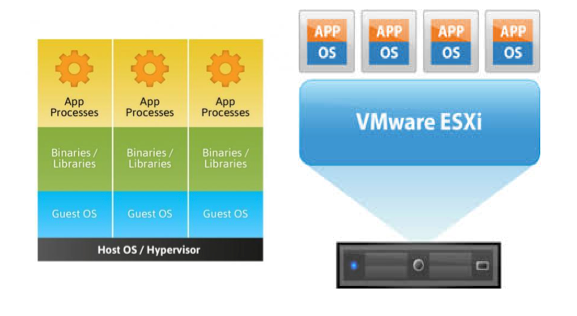
\includegraphics[width=1\textwidth]{images/virtualize-hyper.png}
  \caption
    [Virtualization based on hypervisor]
    {Virtualization based on hypervisor \cite{linuxcontainers}}
  \label{fig:virtualize-hyper}
\end{figure}

\begin{figure}[htb]\centering
  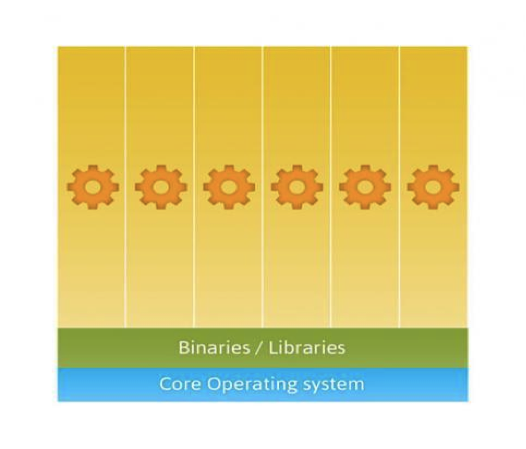
\includegraphics[width=1\textwidth]{images/virtualize-container.png}
  \caption
    [Virtualization based on containers]
    {Virtualization based on containers \cite{linuxcontainers}}
  \label{fig:virtualize-container}
\end{figure}

\chapter{What is Docker?}
Docker is an open-source platform for developing, deploying and running applications. Docker allows to separate applications from infrastructure using environment virtualization, which is empowered by virtualization support  in kernel and by tools that help to manage and deploy applications. Containers are used again, but they are not as independent as OpenVZ containers for example. Docker uses containerization support in kernel, so applications share kernel with the host machine. This makes containers more lightweight, faster to run and portable. Docker allows more advantages thanks to it is wrapping basic kernel virtualization

\section{Docker architecture}
Docker daemon runs on the host machine and manages all Docker images and containers. Docker client communicates with this daemon to create images and to upload them on Docker registry. The figure \ref{fig:docker-architecture} shows the whole concept of it.

\subsection{Docker image}
Docker image is a read-only template. It contains a chosen operating system and a set of installed applications. Images used to run simple binary program can also start from scratch.

\subsection{Docker container}
Docker container is a structure holding everything what application may need to run. Each container is based on an image. There can be multiple containers based on the same image, all of them can be started, stopped, moved or deleted individually and users can attach to any of them. Containers provide an isolated and a secure platform for applications.

\subsection{Docker registry}
Docker registry is a server-side application holding images. It is a storage, where clients can push their images so anyone can pull them and run containers based on them.

\begin{figure}[htb]\centering
  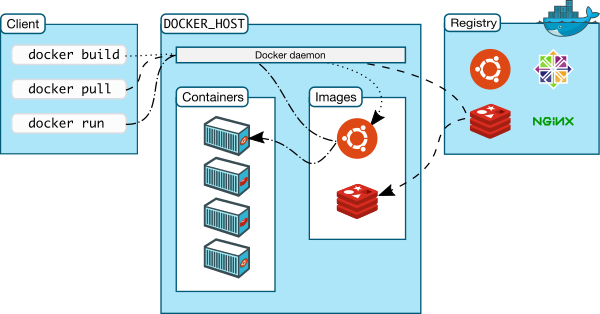
\includegraphics[width=1\textwidth]{images/dockerarchitecture.png}
  \caption
    [Docker architecture]
    {Docker architecture \cite{dockerdocs}}
  \label{fig:docker-architecture}
\end{figure}
\chapter{Kubernetes basic concepts}\label{chapter:kubernetes-basic-concepts}

\section{Pod}
In Kubernetes all containers are run in so called pods. Pod is a package of more containers (or just one) which logically belong to each other (for example application server and its proxy). It is against Docker principle to run more processes in a single container, but proxy and server have to be on same server so they can communicate via localhost and don’t overload the network. Pod is the basic building block so it is provided that containers belonging to it will be run together on the same machine. Scaling is done with whole pods.

\section{Volume}
In Docker a volume is a directory on a filesystem or in another container. Kubernetes volumes are more abstract. Kubernetes volume has a defined service life, which is the same as the service life of the pod which requested it. Pod may contain none or more volumes and each container in it has to define where the volume should be mounted.

\section{Replication controller}
Replication controller (RC) specifies the amount of pods to run at the same time. If there is fewer, it creates new ones, if there is too many, it stops some. RC keeps running exactly the same instances of pods as the maintainer wants to. 

\section{Service}
Pods in Kubernetes may start and quit as the replication controller settle. Each pod has its own IP address which can change during time so it is better not to rely on it, because pod can be moved to another machine. Which leads to a problem: what if a pod (and container in it) needs to communicate with another one? Here comes the Kubernetes service. It is an abstraction layer which defines a logical set of pods and rules for accessing them. Sometimes it is called a micro-service as well. As an example I~can mention a backend service which is running in 3 instances. The frontend does not care about which one of them it will be communicating with.
\chapter{Kubernetes architecture}

\section{Etcd}
Etcd is a distributed, consistent key-value store for shared configuration and service discovery \cite{etcd}.	

\section{API server}
The Kubernetes API server validates and configures data for the API objects which include pods, services, replication controllers, and others. The API Server services REST operations and provides the frontend to the cluster shared state through which all other components interact. \cite{kubernetesdoc}

\section{Kubelet}
Another very important part of Kubernetes is Kubelet. Kubelet is an agent running on every node and it provides starting and stopping containers.

\section{Kube-proxy}
Every node in Kubernetes cluster has its own kube-proxy. This application watches the Kubernetes master node and in case of adding or deleting a service it will open or close ports (even randomly chosen) on the local node. Each connection is then forwarded to the right pod.

\begin{figure}[htb]\centering
  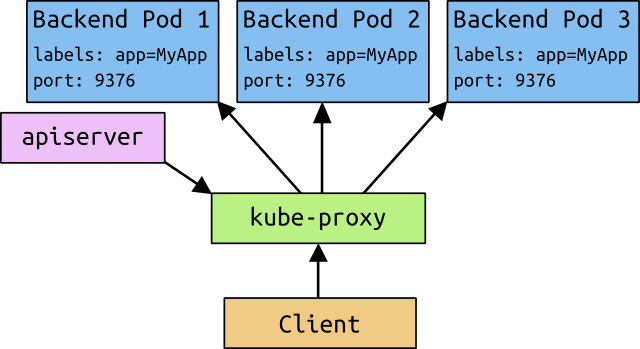
\includegraphics[width=1\textwidth]{images/services-overview.png}
  \caption
    [Service overview in Kubernetes]
    {Service overview in Kubernetes \cite{kubernetesdoc}}
  \label{fig:services-overview}
\end{figure}

\section{Controller manager}
The Kubernetes controller manager is a daemon that embeds the core control loops shipped with Kubernetes. In robotics and automation applications, a control loop is a non-terminating loop that regulates the state of the system. In Kubernetes, a controller is a control loop that watches the shared state of the cluster through the API server and makes changes in order to move the current state towards the desired state. Examples of controllers currently shipped with Kubernetes are the replication controller, endpoint controller, namespace controller, and service account controller. \cite{kubernetesdoc}

\section{Scheduler}
The Kubernetes scheduler runs as a process alongside other master components such as the API server. Its interface to the API server is to watch for pods with an empty \lstinline{PodSpec.NodeName}, and for each pod, it posts a binding indicating where the pod should be scheduled.

\begin{figure}[htb]\centering
  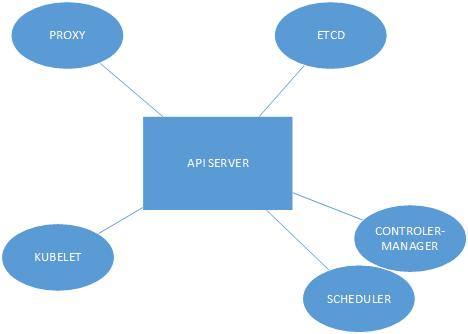
\includegraphics[width=1\textwidth]{images/kubernetes-services.png}
  \caption
    [Kubernetes services interconnection]
    {Kubernetes services interconnection \cite{tomkukral}}
  \label{fig:kubernetes-services}
\end{figure}

\section{Node}
There are two types of nodes in a cluster: the master node and the worker nodes, formerly known as minions. On the master node the API server, the scheduler and the controller manager are running together with etcd and possibly flannel. Each node runs Kubelet and optionally flannel. Using Docker for those main Kubernetes parts, the final structure of the nodes is as follows in the figure \ref{fig:kubernetes-docker-nodes}.

\begin{figure}[htb]\centering
  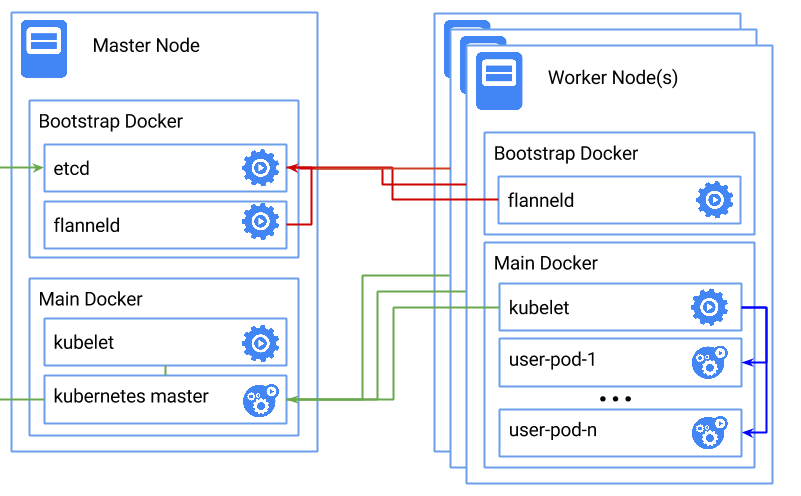
\includegraphics[width=1\textwidth]{images/k8s-docker-nodes.png}
  \caption
    [Kubernetes nodes]
    {Kubernetes nodes \cite{kubernetes-docker-multinode}}
  \label{fig:kubernetes-docker-nodes}
\end{figure}

               
\chapter{Possible problems with Kubernetes in Seznam.cz}

This chapter summarizes what we have to focus on in Seznam.cz so we can build and maintain a Kubernetes cluster.

\section{Docker registry}
We have to build our own Docker registry with a support for authentication so it is clear who and when pushed a certain Docker image and who is responsible for it in case of problems. Next we have to run Docker registries for developers both in testing and production environment. Images have to be mirrored from one to another registry. Production registry has to be in each data centre and it has to be a high availability service because if a whole data centre depends on a single server with Docker registry and the server fails (which it will if a whole data centre starts pulling images from it at once), it will be impossible to run new applications.

\section{Secrets distribution}
How to share passwords, certificates and other secrets which are different in development and test/production environment and which cannot be available outside of the containers that need them? Moreover, the production secrets are known only to administrators, so there has to be an easy way how to put secrets into containers without compiling them in images. Kubernetes has a technique for it and it calls it Kubernetes secrets. It has to be examined more closely and run in Seznam.cz conditions and environments.

\section{Logging}
Logging is a very huge problem. Actually most of our applications are creating debug logs, which are saved on the file system. In case of switching pods among servers there has to be a log collection and their transfer to a central storage and it has to be done so that applications don’t get overloaded.

Beyond debug logs we also create so called business logs which are sensitive and cannot be lost because there are more calculations over them.

And there are also third party logs such as access logs from Nginx \cite{nginx} or Apache \cite{apache} and many more. Their collection has to be done as well as gathering server side statistics (CPU load, etc.). There is a Kafka cluster at Seznam.cz for this task, which can also run support jobs to forward the logs to specific databases (Elasticsearch \cite{elasticsearch}, HDFS \cite{hdfs}, \ldots).

Problems may occur with long running applications that generate large log files unless there is a logrotate running. Cron or logrotate \cite{logrotate} do not belong to Docker images, because Docker principle is to run only one application in each container.

\section{Security}
At the moment administrators are taking care of host machines and virtual machines running on them and developers only deploy applications in form of Debian packages. When a  security issue is discovered (like Heartbleed \cite{heartbleed} for example) administrator is able to maintain it and fix whatever it needs on the host machine or in specific virtual machine. When developers will deploy Docker images with operating system inside, fixing such images in case of security issue needs to be solved. Definitely we cannot rely that developers will rebuilt images in a few minutes. In case of automatically built images the whole environment for it has to be built and we also the authorization have to be solved sufficiently.

\section{Monitoring}
We need to monitor nodes in cluster and also applications and containers in Kubernetes. We are testing Prometheus \cite{prometheus} for metrics collection, while monitoring what is running where is built in Kubernetes itself.

\section{Static content of websites}
When deploying a website, there are always at least 2 versions running at the moment. The old one, where most of the traffic is going to, and the new one. The problem comes when user sends a request and the new version responds. User will receive a HTML code with links to JavaScript and CSS files and send a request for these files to the data centre. The load balancer and other services on the way may point this request to the pod with the old version of the website so none or wrong files will be downloaded and user will see the page with errors (or nothing at all).

At the moment we are deploying static content of websites first and it is installed on all machines. Static content is versioned in its path, so requests for it are always successful. Than one machine is removed from the pool (and waits until all currently opened connections are done) and it is replaced with a new version. This ensures that downloading static content never fails. However, this procedure will no longer be available in Kubernetes.

\begin{flushleft}
These are the problems which I~have to find solution for.
\end{flushleft} 

\chapter{Running Kubernetes}

I~will run Kubernetes on 3 testing machines. First decision I~have to make is which operating system I~will use. Since almost all machines in Seznam.cz data centres are running Debian I~will use it as well on my testing cluster and I~will install its newest stable version Jessie. There are Linux distributions made especially for Kubernetes like Fedora Atomic \cite{fedora-atomic}, but as our administrators have many years of experience with Debian, it will be better to use it instead of changing architecture to cloud and changing Linux distribution at the same time.

Another decision that has to be make is about networking.

\section{Networking in Kubernetes}

Kubernetes assumes that pods can communicate with other pods, regardless of which host they land on. They give every pod its own IP address so I~do not need to explicitly create links between pods. This creates a clean, backwards-compatible model where pods can be treated much like VMs or physical hosts from the perspective of port allocation, naming, service discovery, load balancing, application configuration, and migration. \cite{kubernetesdoc}

\subsection{Docker model}
Before discussing the Kubernetes approach to networking, it is worthwhile to review the ``normal" way that networking works with Docker. By default, Docker uses host-private networking. It creates a virtual bridge, called docker0 by default, and allocates a subnet from one of the private address blocks defined in RFC1918 \cite{rfc1918} for that bridge. For each container that Docker creates, it allocates a virtual Ethernet device (called veth) which is attached to the bridge. The veth is mapped to appear as eth0 in the container, using Linux namespaces. The in-container eth0 interface is given an IP address from the bridge’s address range.

The result is that Docker containers can talk to other containers only if they are on the same machine (and thus the same virtual bridge). Containers on different machines cannot reach each other –- in fact they may end up with the exact same network ranges and IP addresses.

In order for Docker containers to communicate across nodes, they must be allocated ports on the machine’s own IP address, which are then forwarded or proxied to the containers. This obviously means that containers must either coordinate which ports they use very carefully or else be allocated ports dynamically. \cite{kubernetes-networking}

\subsection{Kubernetes model} 
Coordinating ports across multiple developers is very difficult to do at scale and exposes users to cluster-level issues outside of their control. Dynamic port allocation brings a lot of complications to the system – every application has to take ports as flags, the API servers have to know how to insert dynamic port numbers into configuration blocks, services have to know how to find each other, etc. Rather than deal with this, Kubernetes takes a different approach.

Kubernetes imposes the following fundamental requirements on any networking implementation (barring any intentional network segmentation policies):

\begin{itemize}
\item	all containers can communicate with all other containers without NAT
\item	all nodes can communicate with all containers (and vice-versa) without NAT
\item	the IP that a container sees itself as is the same IP that others see it as
\end{itemize}

In reality, Kubernetes applies IP addresses at the pod scope -- containers within a pod share their network namespaces -- including their IP address. This means that containers within a pod can all reach each other’s ports on localhost.

This networking mode is implemented in many different ways. The basic one and the one which is mentioned in documentation of Kubernetes is flannel. \cite{kubernetes-networking}

\subsubsection{Flannel}
Flannel is a virtual network that gives each host a subnet for use with container runtimes.

Platforms like Google's Kubernetes assume that each container (pod) has a unique, routable IP inside the cluster. The advantage of this model is that it reduces the complexity of doing port mapping.

Flannel runs an agent, flanneld, on each host and is responsible for allocating a subnet lease out of a preconfigured address space. Flannel uses etcd to store the network configuration, allocated subnets, and auxiliary data (such as hosts' IP addresses). The forwarding of packets is achieved using one of several strategies that are known as backends. The simplest backend is UDP and uses a TUN device to encapsulate every IP fragment in a UDP packet, forming an overlay network. The following diagram \ref{fig:flannel} demonstrates the path a packet takes as it traverses the overlay network. \cite{flannel}
                              
\begin{figure}[htb]\centering
  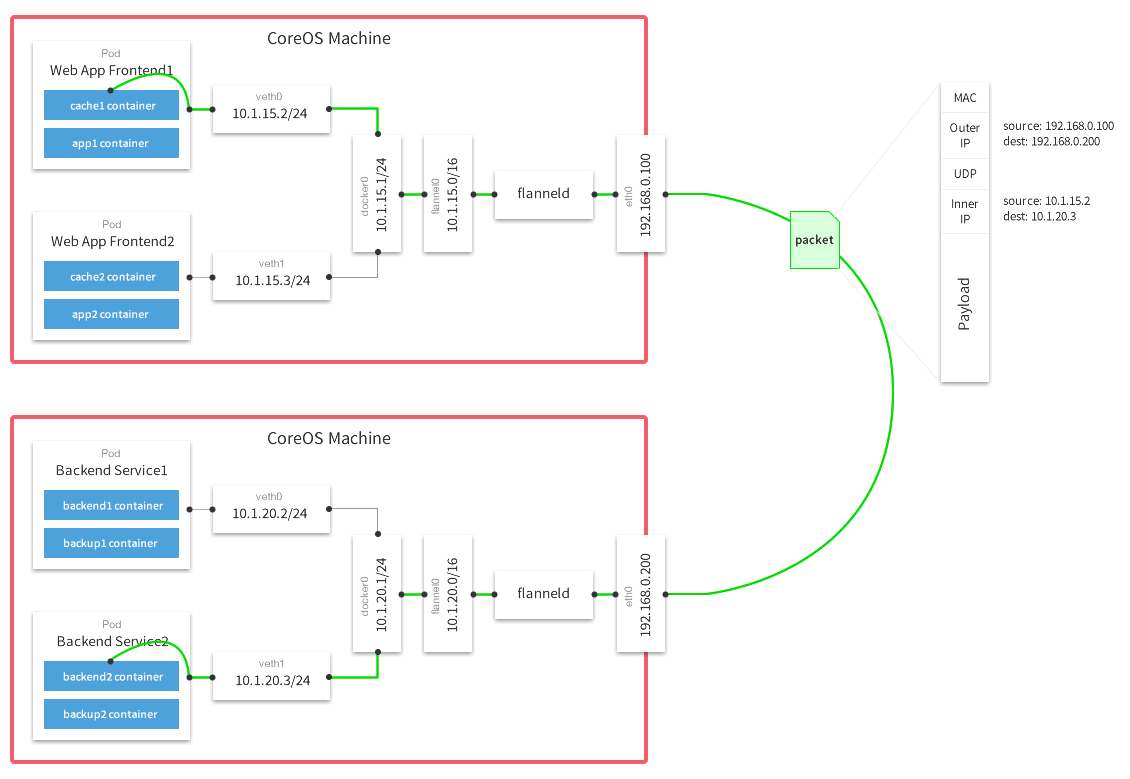
\includegraphics[width=1\textwidth]{images/flannel.png}
  \caption
    [The path of a packet in flannel network]
    {The path of a packet in flannel network \cite{flannel}}
  \label{fig:flannel}
\end{figure}

Flannel is simple to start up but there can be some overhead expected. It is needed to test how big overhead it will be. Another big disadvantage of flannel is that it is not multitenant and so there is no way how to define any rules who can communicate with whom and who can’t. In practice that means everyone sees everyone. For introducing cloud at Seznam.cz it can be sufficient but in the future this needs to be solved more properly so there can be policies defining restricted access to sensitive services.

\subsubsection{Calico}

Next networking option is Calico. Calico provides a highly scalable networking solution for connecting data center workloads (containers, VMs, or bare metal). It is based on the same scalable IP networking principles as the internet: providing connectivity using a pure Layer 3 approach. Calico can be deployed without encapsulation or overlays to provide high performance at massive scales.

When using Calico networking in containerized environments, each container gets its own IP address and fine grain security policy. A~calico-node service runs on each node which handles all of the necessary IP routing, installation of policy rules, and distribution of routes across the cluster of nodes.  \cite{calico}

Calico has even a section dedicated for Kubernetes in their manual \cite{calico-kubernetes}. They state that thanks to that there is no overlay, Calico will be faster than technologies that use overlay, such as flannel. Calico is using the Bird \cite{bird} system for route distribution around the network.

\subsubsection{OpenContrail} 

On the meeting with company tcp cloud \cite{tcpcloud} technology OpenContrail was discussed \cite{tcpcloud-opencontrail}. OpenContrail is a network virtualization platform for the cloud. It has been designed with scale out in mind  \cite{opencontrail}. OpenContrail is a representative of SDN (software defined networking) and it offers to define custom policies of containers communication thanks to label system in Kubernetes. It will be worth it to examine whether this technology fits for Seznam.cz needs and environment.

\section{Starting cluster}
From listed options of network management I~decided to start with a simple one: the flannel. This thesis should create a proof of concept that it is possible to maintain Kubernetes in Seznam.cz. I~want to create a testing application and an example Kubernetes cluster where I~solve all potential problem described in the previous chapter and then I~give this to our administrators who may test it further as they want to.

Running flannel containers needs privileged permissions but user defined pods and their containers should not ever have such permissions. So the best way how to achieve this behaviour is to start two separate Docker daemons where one will allow to create privileged containers and the second one won’t.

Starting Docker on Seznam.cz corporate machines brought a couple of problems that must be solved first. From Seznam.cz system preinstaller in \lstinline{/etc/network/interfaces} all routes to private IPs are routed via eth0 interface which cases that Docker could not find and private IP range free for its purposes. This can be simply solved by freeing an IP range and restarting network service together with Docker daemon.

Next issue that occured was a little bit tougher. In the Docker log I~found that no chain exists for an iptables rule which Docker wants to set. After consulting this problem with my team leader it proved to be caused by missing kernel modul \lstinline{xt_conntrack}. After adding this module to kernel Docker daemon finally started.

In the Docker log I~also found a warning that cgroup memory is not allowed and that could possibly cause Kubernetes to not work properly with pod memory limitation. I~added \lstinline{GRUB_CMDLINE_LINUX="cgroup_enable=memory swapaccount=1"} to the \lstinline{/etc/default/grub} file and updated grub.

With the Docker daemon running I~could start Kubernetes. As was shown in the \nameref{chapter:kubernetes-basic-concepts} chapter, the master node has to have API server, scheduler, proxy, kubelet, controller-manager and flannel running in a separate Docker daemon.

The first step is to create a bootstrapped daemon. The second is to run etcd. I~used \lstinline{gcr.io/google_containers/etcd-amd64} image. The third is to setup flannel. I~also used a prebuilt image, this time \lstinline{quay.io/coreos/flannel}. Finally the last step is to start kubelet. Kubernetes offers prebuilt Docker image with all its components included called \lstinline{gcr.io/google_containers/hyperkube-amd64}. From the hyperkube image the kubelet is called and in configuration of the kubelet there is a set of static pods that should be created. The hyperkube firstly creates those pods and then starts the kubelet. Those pods are the scheduler, the API server, the controller-manager and the kube-proxy.

I~have prepared a script where this whole configuration is scripted and which may be called with the following single line: \lstinline{./kube.sh start-master} You can also specify which components should be started.

Now the worker has to be set. The configuration is similar only there is not so many components to run. The first step is also to create a bootstrapped daemon, then the flannel and the kubelet are started, respectively. The kubelet is configured to run only kube-proxy.

Now adding a new worker node to the cluster is very simple. Install the system, fix problems described earlier and then upload a script and run .\lstinline{/kube.sh start-worker}. This system may be automated with ansible \cite{ansible} for example but this is a task for our administrators.

Also there are other possibilities how to run this Kubernetes model. The kubelet can be installed on bare-metal and not be dockerized and the same applies to the flannel. But it really is just a matter of personal preferences.

The cluster is now fully functional and pods may start to be distributed.

\begin{figure}[htb]\centering
  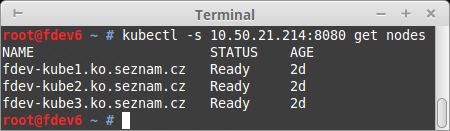
\includegraphics[width=0.95\textwidth]{images/kubectl_get_nodes.png}
  \caption
    {Screenshot of \lstinline{kubectl get nodes} output}
  \label{fig:kubectl-get-nodes}
\end{figure}


\chapter{Docker registry}

The Registry is a stateless, highly scalable server side application that stores and lets you distribute Docker images. \cite{docker-registry}

The Registry is the only reasonable way how to distribute Docker images inside a network. When a developer creates new image with his application, there are 2 ways how to get it to production. The first one is to do it through a Dockerfile. The second one is using Docker image. In the future it would be nice to have a whole system, where you only put a new Dockerfile (let’s say simply by merging your dev branch with the new Dockerfile to the master branch in Git) and the system will then build your image, tag it properly and upload it to the Docker registry. This is a state we want to achieve eventually, but it currently takes more work than we can afford to build a system like this.

So the second way is that Deznam.cz will have to create a Docker registry, where developers can push their images and then send tickets to administrator to get them in production. So I~have to study the Docker registry more deeply. The Registry is an application that you can run on server. Then every developer have to tag his image with server name and port on which the registry is running and append his own name. In Seznam.cz we are prefixing each name of application with the department name and the ``szn" prefix. For example \lstinline{szn-fulltext-APP_NAME}. So basically now each developer will have to tag his image similarly like that: \lstinline{REGISTRY_URL /fulltext/APP_NAME} and push it. The Registry URL has to be easy to remember and we need to be sure it does not cause conflict in the future. You also have to define which images will be included in the Kubernetes pod and those pod definitions have to be created in a cooperation of developers with administrators. And if there are different names for the registry in development, staging and production environment those pod definitions will have to be updated each time which might easily lead to mistakes.

We have to create development, staging and production Docker registry servers where images will be stored. The development registry can be a standard server with a large disk space because many versions of images will be stored here. Developers will have unlimited access to it via the Docker command line tool and no special policy will be defined here.

We cannot have the dev registry with authentication because when pushing new image to registry you would have to set password. As the credentials are stored in \lstinline{\$HOME/.dockercfg} and every developer in our development environment has root privileges, such practice would be insecure and untrusty.

After successfully creating an image and uploading to the dev server, the developer will have to send a request to an administrator to deploy it. In Seznam.cz we have a custom request tracker and when someone want to deploy something, we have to send a RT ticket with a number of the particular Debian package version. The only difference with Docker would be that the developer will  send an image signature hash created by Docker. This way there will always be a possibility to authenticate possible and the developer who sent the ticket will be responsible for his image.

The administrator will then pull the image from the dev registry and push it to the staging registry and then to the production registry.

When Kubernetes starts a new pod, the Kubernetes master node downloads the image from registry (if it’s not present already) and run it. This logic makes the registry server a bottleneck for the entire cluster. When the master node cannot pull from the registry server, the application won’t start. And even when app is running, if the registry server fails and then Kubernetes decides to migrate this pod from one server to another because of load balancing or something else, application can easily become unavailable. That means that Seznam.cz’s Docker registry in the production environment has to run on high availability servers.

The Docker registry is an application which provides an API for clients and the storage itself is delegated to drivers. The default driver is posix filesystem.  As is said in the manual, this default driver is fine for small deployments and in our conditions will be fine for development environment where physical hard drivers will be mirrored. Development registry server does not have to be high availability and there is always a way how to start custom registry even on local machine.

The Docker registry storage drivers provided are \cite{docker-registry-storages}:

\begin{itemize}
  \item \textbf{inmemory}: A~temporary storage driver using a local inmemory map. This exists solely for reference and testing.
  \item \textbf{filesystem}: A~local storage driver configured to use a directory tree in the local filesystem.
  \item \textbf{s3}: A~driver storing objects in an Amazon Simple Storage Solution (S3) bucket.
  \item \textbf{azure}: A~driver storing objects in Microsoft Azure Blob Storage.
  \item \textbf{rados}: A~driver storing objects in a Ceph Object Storage pool.
  \item \textbf{swift}: A~driver storing objects in Openstack Swift.
  \item \textbf{oss}: A~driver storing objects in Aliyun OSS.
  \item \textbf{gcs}: A~driver storing objects in a Google Cloud Storage bucket.
\end{itemize}


From all these drivers provided the only two options we can use are rados, with Ceph Object Storage and swift with Openstack Swift storage. And because in Seznam.cz there are administrators who are well acquainted with the technology of Swift, we decided that for the production registry we will use swift as a storage driver.

So the final model is shown in the following figure \ref{fig:seznam-docker-registry}.
                
\begin{figure}[htb]\centering
  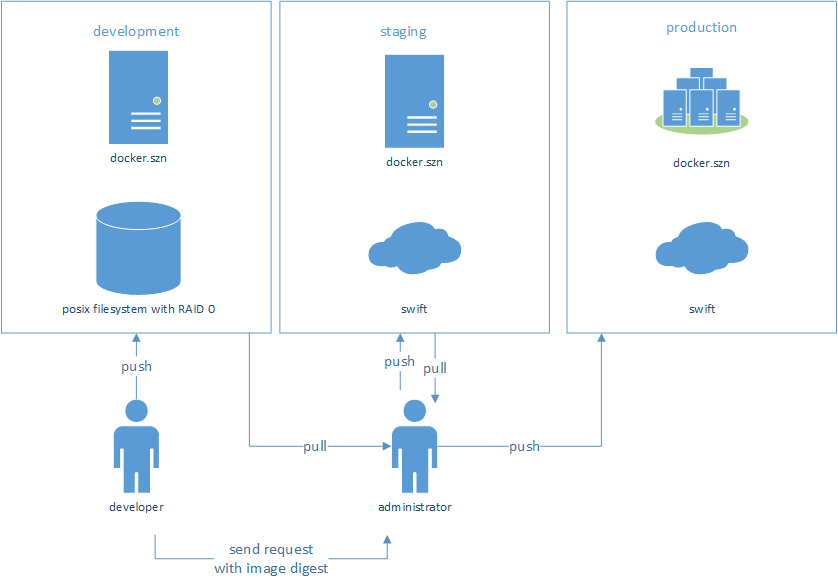
\includegraphics[width=1\textwidth]{images/registry.png}
  \caption
    {Seznam.cz Docker registry architecture}
  \label{fig:seznam-docker-registry}
\end{figure}

\chapter{Secrets distribution}

Kubernetes has a mechanism for storing secrets –- passwords, keys, certificates, etc. Unsurprisingly, they call it the secret.

Objects of the type secret are intended to hold sensitive information, such as passwords, OAuth tokens, and ssh keys. Putting this information in a secret is safer and more flexible than putting it verbatim in a pod definition or in a Docker image. \cite{secrets} 

Using secrets is safer than putting those sensitive information somewhere else, like directly to Docker images, to the file system mounted as a volume, to environment variables, etc. The main idea of the secret is to keep them centralized somewhere safe and distribute them only to those master nodes which need them. And also of course to have them on the master node only as long as necessary. For those purposes Kubernetes are using etcd as a persistent centralized storage that ensures high availability through peer-to-peer synchronization between machines. Each master node has a Kubelet daemon which can ask secrets API server for a secret. Communication from the master node to the etcd is encrypted. The Etcd sends the secret object to the master as a base64 encoded string. The size of the secret is limited to 1 MB and the master node will save the secret value to its memory, Not to the file system, which means that when the master node crashes and its memory is deleted, no secret can be compromised. The Kubelet then mounts the secret value to containers in the pod which requested it as a tmpfs filesystem. Secrets in the etcd are divided into namespaces and only pods from the same namespace can ask for them. It is the main responsibility of administrators to check the pod’s namespace when they accept it and deploy it to a running cluster.

After consulting the Kubernetes secret with our administrators we agreed that it would be nice to have the same feature for the current virtualization technologies (LXC and OpenVZ containers). The logic can be almost the same as Kubernetes have. And because the Kubelet is a standalone binary which can be called even without Kubernetes and the etcd is also an independent component, we decided to build a secrets distribution system for the current solutions at Seznam.cz. Each LXC container or OpenVZ virtual machine will have the Kubelet binary in its image. After installing a new virtual machine, the administrator will add a certificate signed by his team’s certification authority, which will be configured at etcd so it can request only secrets belonging to his team. There can be special one way certificates for highly sensitive data as well. After the virtual machine starts, it will start monitoring a known file, such as \lstinline{/www/secrets/request.json}, where applications or even the administrator of the virtual machine have to specify which secrets are requested. The Kubelet then asks the etcd for them and saves them via tmpfs to a known place such as \lstinline{/www/secrets/data/}. New applications have to be edited for those new features.

The main advantages of this approach is that all secrets are saved at one safe plac with a high availability for the whole company infrastructure and both master and virtual machines do not keep secrets for ever but only on a temporary file system in their memory.

\chapter{Logging}

Logging is quite a big problem in almost every system. At the moment in Seznam.cz we have a special library called dbglog which is used for logging from C/C++ and Python. This library is also open sourced \cite{dbglog}. You can configure it to log to stderr or to a file. It simply formats the message with data arguments add a general info, like file from which the log message has been called, the line number, the function name, the log level, current time and so on.

The text files take up a lot of space, so we had to think about storing information in a binary form or even compressed. Another idea was to store logs not as simple strings but in a structured form. That would be very helpful for a basic analysis of these debug logs, for example to check the number of records processed etc. We started to develop a complex logging solution quite a while ago. I~implemented a library for storing data to binary files. The library is in Go and uses the Apache Kafka \cite{kafka} file format. Picking the Kafka file format was quite an easy decision, as we wanted to use the Kafka cluster as a logging service where all our applications will send their logs. Then we can decide which logs go to the Elasticsearch \cite{elasticsearch} for a human analysis and which will go to the HDFS \cite{hdfs} for permanent storage and time consuming calculations. And of course in the future more approaches can come. Kafka file format also supports compression and storing partition key in each message.

A~very common problem with logging into file system is rotating files. There are many approaches for this, but logrotate or another similar daemon running in the background is not the way we want to go in Docker. The Docker principle is to have only one process in one container. Sure you can run logrotate in another container in pod and send signals from one container to the other, but that’s generally not a good idea. That’s why the library for storing logs into file system also supports file rotation.

So at the moment I~have solved the problem with file rotation and storing files from our applications. But how to deal with logs from any third part application? Actually the answer is very easy as well. Does the application support logging to stderr? If so, just make use of it and throug a pipeline to send the stream to stdin for another application which will simply save each line into my library. If stderr is not an option (for example nginx), does the application support syslog interface? If so, do exactly the same, only that the application which reads it will have to expose the syslog interface.

So now I~have the files stored at the file system. How to send them to Kafka for further processing? This simple task proved to be quite tricky. There are several daemons which read files and send them somewhere. Kubernetes also have one of them.

\section{FluentD}

Fluentd is an open source data collector for a unified logging layer. The Fluentd allows to unify data collection and consumption for a better use and understanding of data \cite{fluentd}.

\begin{figure}[htb]\centering
  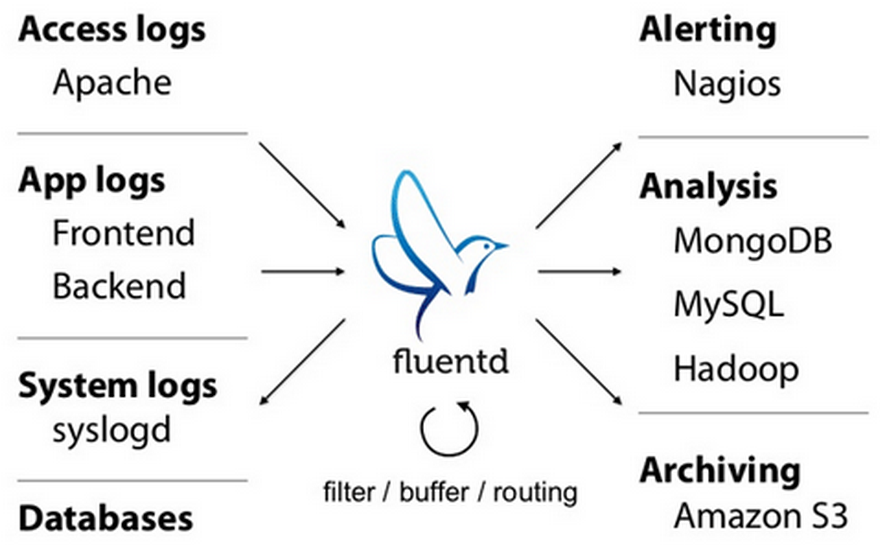
\includegraphics[width=1\textwidth]{images/fluentd-architecture.png}
  \caption
    [Fluentd]
    {Fluentd \cite{fluentd}}
  \label{fig:fluentd}
\end{figure}
 
The Fluentd is natively implemented in Kubernetes but there is a couple of problems. The first one is that plugins for The Fluentd are written in Ruby \cite{ruby}, which is not used in Seznam.cz, so writing a custom plugin could become an issue. And we already know we would need at least one custom input plugin for reading the Kafka file format. The second problem is that in the default configuration the Fluentd reads from the input file, stores those data in a memory buffer and tries to send them to Kafka. When the Fluentd, its pod or even the whole node fails, the data are lost and when it starts again it does not know about the power cut and it starts from the last known position in the file. This all means that the Fluentd is not an option for us.

\section{Logstash}
Logstash is a tool for managing events and logs. It can be used to collect logs, parse them, and store them for later use (e.g. for searching) \cite{logstash}.
 
Logstash plugins are written in JRuby so it’s almost the same as with Fluentd. We tried to use Logstash in the current conditions at Seznam.cz but it completely failed because of memory demands. Logstash is written in Ruby but runs under JVM, so its memory demands are huge. We also wanted to have one log forwarder from the file system to the Kafka for each pod so that the failure of one pod won’t affect other pods and with Logstash’s memory usage this is not possible.
    
\section{Heka}
Heka \cite{heka} is written in Go, its plugins are written in Go and that is an advantage over Logstash or Fluentd. Heka also supports sandboxed Lua for filter scripting without the need to recompile Heka. There are plugins for Apache Kafka, Elasticsearch and many other outputs. That’s why I~started to examine Heka more closely.

Heka is a heavily plugin based system. There are six different types of Heka plugins \cite{heka}:

\begin{description}
  \item[Inputs] Input plugins acquire data from the outside world and inject it into the Heka pipeline. They can do this by reading files from a file system, actively making network connections to acquire data from remote servers, listening on a network socket for external actors to push data in, launching processes on the local system to gather arbitrary data, or any other mechanism.
  \item[Splitters] Splitter plugins receive the data that is being acquired by an input plugin and slice it up into individual records.
  \item[Decoders] Decoder plugins convert data that comes in through the Input plugins to Heka’s internal Message data structure. Typically decoders are responsible for any parsing, deserializing, or extracting of structure from unstructured data that needs to happen.
  \item[Filters] Filter plugins are Heka’s processing engines. They are configured to receive messages matching certain specific characteristics (using Heka’s Message Matcher Syntax) and are able to perform arbitrary monitoring, aggregation, and/or processing of the data. Filters are also able to generate new messages that can be reinjected into the Heka pipeline, such as summary messages containing aggregate data, notification messages in cases where suspicious anomalies are detected, or circular buffer data messages that will show up as real time graphs in Heka’s dashboard. 
  \item[Encoders] Encoder plugins are the inverse of Decoders. They generate arbitrary byte streams using data extracted from Heka Message structs. Encoders are embedded within Output plugins; Encoders handle the serialization, Outputs handle the details of interacting with the outside world.
  \item[Outputs] Output plugins send data that has been serialized by an Encoder to some external destination. They handle all of the details of interacting with the network, filesystem, or any other outside resource. They are, like Filters, configured using Heka’s Message Matcher Syntax so they will only receive and deliver messages matching certain characteristics.
\end{description}

I~developed a custom splitter plugin and a custom decoder in Go, which are able to split and decode data from the Kafka file format. So the default Heka plugin -- Logstream Input -- reads bytes from the Kafka files, the Kafkalog splitter and the Kafkalog decoder create Heka messages which are send through the filters to a simple encoder and to the Kafka output.

When Kafka ran, everything seemed fine and worked as expected. The problems started when I~stressed Kafka. I~shutdown some of the brokers and watched how Heka can handle it. Heka noticed that one or more Kafka brokers were down and the rest was in the middle of the leader election, but it didn’t stop trying to send messages. It slowed down, because of the timeouts that occurred, but after a while the message that cannot be delivered to Kafka is dropped down and the Input plugin reads new bytes from the file. I~tried to simulate Heka failure, simply by Linux kill command.

The Logstream input plugin keeps a journal file. In the journal there is the file name, the offset of the last read message and the control hash. But the problem is, that input plugins do not cooperate with outputs. Heka is highly expandable with plugins. One input can generate message to Heka’s pipeline and more outputs can read them and do something with them. Filters can drop messages or create new messages so there is no simple way to synchronize the input and the output plugin. Which means there is a risk of losing messages.
 
I~did a research about Heka’s reliability and found a couple of some e-mails and discussions where the Heka authors are saying that 100 \% reliability was never their goal. But we need it at Seznam.cz as we can’t say that some logs will possibly be lost. So I~try to fix this.

The Kafka output plugin uses the Sarama library from Shopify \cite{shopify} to communicate with Kafka. There is a synchronous and an asynchronous Kafka producer. In the output plugin the asynchronous one is used. The asynchronous producer is faster, because it does not wait for errors or success confirmation. All messages are handled in separate goroutines\footnote{A goroutine is a lightweight thread managed by the Go runtime \cite{goroutine}.}. Producer errors are handled in output plugin, but only to be logged and dropped down. I~fixed this with a special error channel addition. When an error occurs, it is sent to the error channel and the main goroutine which process Heka messages starts fixing it. When there is an error I~don’t want to process any other messages from the Heka pipeline, the backpressure is desirable. I~create one extra synchronous Kafka producer with exactly the same configuration as the main (async) one and the error is sent through it. The maximum number of attempts is configurable and can even be set to infinity. Dealing with the error through the synchronous producer will not read from the main message channel, which can fill up eventually. This causes a backpressure and Heka will stop in such case (of course, only under the condition that no other output processes the input messages).

I~have tested this by writing a Kafka consumer in Python and uploading files with a few millions of numbered messages. The consumer reads everything from the special topic and looks for holes and duplicates in sorted sequence of messages. I~randomly shut down Kafka brokers, even whole Kafka, simulating packet lost with Linux iptables DROP directives and watched consumer’s statistics. It turned out that with a few millions of messages there is a few thousands of duplicates but no miss. Duplicates can also be caused by consumer, because Kafka’s philosophy is to deliver each message at least once. And duplicates are no problem for us, because we can easily discover them. This fix seems quite useful and generic, so I~will try to send it to the upstream as a merge request.

Fixing this issue will only try to repeat errors when they occurs. This does not solve the next problem, when Heka input plugin reads something from a file, it confirms the new offset to its journal file and sends the message to the Heka pipeline. If Heka fails now, the memory buffer will be lost and after a new start the input file will seek to the position from the journal file. I~need to figure out how to fix this too. 

The problem is, that one input can be processed by more outputs, and also more inputs can be processed by a single output. The input and the output plugins don’t know about each other. I~think there is not one generic solution for this problem. The best what I~could come out with is the following idea:

\begin{itemize}
  \item Each input plugin will be working as is plus it will be adding filename, offset and its name as fields to the message. 
  \item The output plugin will be also working as is plus it will read the success message from Kafka, confirming that message was delivered to it. Output saves those metadata sent from input to its private variable and once in a while it sends a special message: an acknowledgement consisting from the filename, the offset and the name of the input plugin.
  \item I~will write a new plugin, the Checkpointer, which will consume acknowledgements from the output and save checkpoint files per each input. This plugin has to know which outputs consume messages from which inputs to be able to successfully maintain acknowledgements from more output that consumes from single input.
\end{itemize}

This theoretical idea might be good, but it is unfeasible in practice. The main problem is, that output plugins are not allowed to generate new messages. Also the condition to know about all other plugins is senseless in Heka.

So I~have to update my idea to be implementable in Heka and useful for Seznam.cz. Our applications logs through my library, which rotates file and is using our naming convention: \lstinline{datetime-timezone-rotate_interval-component_name-postfix.szn}. One application can generate more files with different postfix value. For example \lstinline{szn-fulltext-NAME-dbg} and \lstinline{szn-fulltext-NAME-event}. In the log directory, there is a \lstinline{kafkafeeder.yaml} file -- with our generic configuration where to send files, how long to retain them and so on. That means in our conditions it is possible to always have one input for one output. The problem that output plugins are not able to send new messages can be solved by implementing the checkpointer logic right into the Kafka output, so it will be saving checkpoint files to the file system.

There have to be written a new binary, which will start, copy checkpoints to journals, transform Kafkafeeder configuration to a Heka specific configuration format, start Heka with some predefined options, watch checkpoints and data in a separate goroutine and delete old (and successfully uploaded) log files from filesystem.

This solution will be 100 \% reliable but it is also Seznam.cz specific, because our custom binary (let’s call it Kafkafeeder) will transform our custom configuration to the Heka format  and it will create one Input plugin for one Output plugin with a unique name, so checkpoints can be saved and reused as journal files of those Inputs.
 
\subsection{Kafkafeeder}
I~started designing this application in Go. The Kafkafeeder has to:
\begin{itemize} 
  \item	Copy checkpoints to journal directory
  \item	Start Heka daemon (\lstinline{hekad})
  \item	Monitor log directory for changes
    \begin{itemize}
      \item Reload when it finds a new \lstinline{kafkafeeder.yaml} or when an existing one disappears
    \end{itemize}
  \item	Convert the \lstinline{kafkafeeder.yaml} custom configuration to the Heka format and reload hekad 
  \item	Monitor checkpoints and delete old and successfully uploaded logs from the directory
\end{itemize}

The application is made as a five goroutine architecture, where the main goroutine initializes all the necessary objects and starts all other goroutines.

The cleaner goroutine is responsible for removing old logs, which have been successfully sent to Kafka. Successful dispatch may be tracked from checkpoint files generated by heka. All files with their last modification time older than the retention duration in the configuration file will be deleted.

The signal goroutine is waiting for system signals and handles them properly. When \lstinline{SIGTERM} is captured, the main shutdown function is called and the whole application stops safely. When \lstinline{SIGCHLD} signal is captured forked child is dead and so I~have to check if it should be running. If so, a problem occurred and the main shutdown function is called.

The watcher goroutine periodically watches the directory with logs. When \lstinline{kafkafeeder.yaml} file is found it is registered to LogManager object. After all new logs are registered, the keepValid function is called so the LogManager will keep only those records that actually exists. If something was changed, the reload is called.

The hekad goroutine is responsible for copying checkpoint files to the Heka journal files and starting, stopping and checking hekadCmd. Also when the reload is called, the hekad goroutine converts all logs from LogManger to the Heka specific configuration.

HekadCmd is a wrapper around the actual hekad process. This wrapper sends signals to forked process, captures its standard output and error and logs all messages via the internal logger.

\begin{figure}[htb]\centering
  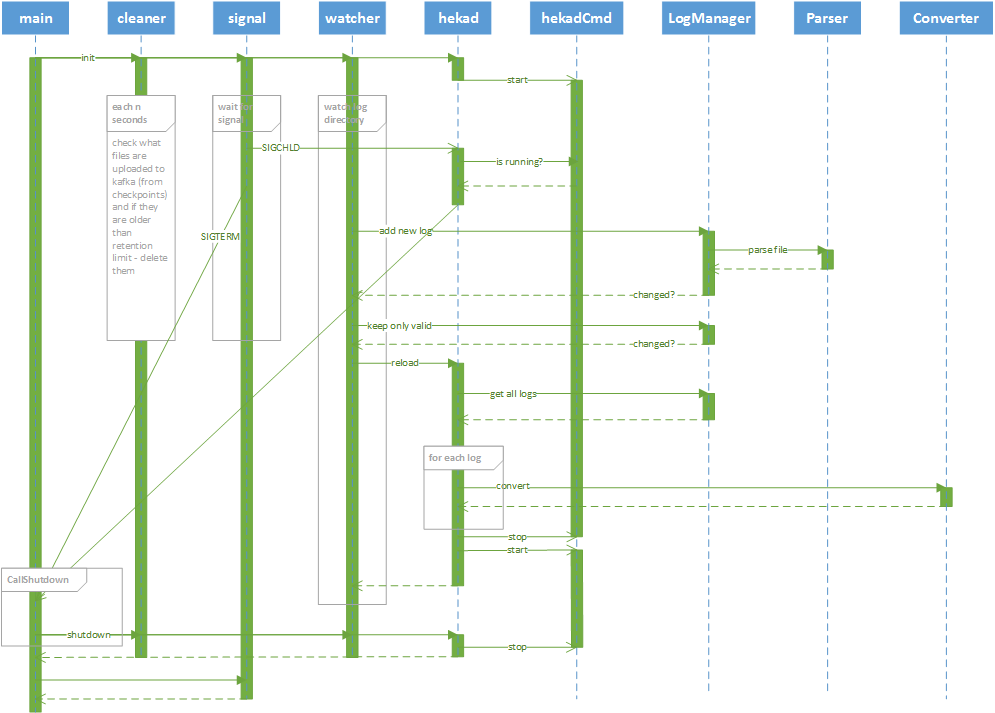
\includegraphics[width=1\textwidth]{images/kafkafeeder.png}
  \caption
    [Kafkafeeder architecture]
    {Kafkafeeder architecture}
  \label{fig:kafkafeeder}
\end{figure}
                            

\chapter{Security}

As was written before, at the moment masters and virtuals in production environment are under the administration of administrators. When a security issue is discovered, they can fix it in a matter of minutes. But on the other hand developers are forced to pack each app into a Debian package. And there are applications from many different corners, Python uses pip \cite{pip} for its packages, nodeJs \cite{nodejs} has npm \cite{npm} repositories, Go is built from source code and so on.

With the advent of Kubernetes it will no longer be sustainable to check if every piece of code in production is packed in a Debian package and uploaded to custom repository, where it can be easily tracked if a newer version with security fixes is released.

Because of that there has to be created a new mechanism how to check
\begin{enumerate}
  \item What is installed and will be running in a Docker image (system, applications, dynamic libraries, \ldots)
  \item Using what and where was it built (gcc version, Go source codes, static libraries, \ldots)
  \item Where is the Docker container running at the moment
\end{enumerate}

Those easily looking conditions are quite hard to satisfy in practice. Seznam.cz at the moment is using custom system called Puzzle where everyone can find on which virtuals is his component running, what packages and their versions are installed on specified virtuals and on what virtuals is installed specified package and version. Those information are delivered to system backend via script called self-checked that have to be installed on each master and is monitoring its virtuals and software installed in it.

After consultation with our security admins we decided that same function is needed also with Docker cluster.

The suggested solution is to create a mechanism that will sniff Docker image during pulling from development registry and pushing it to staging registry and divulge all necessary information about its content. Those information together with image digest will be sent to the Puzzle system API for future tracking. There have to be tracked not only version of debian packages but also pip and other python modules versions, npm packages, Bower \cite{bower} packages\ldots All other packages apart from ours have to be tracked as well. So we will have to build cache server for each of those repositories and run it. When developer wants to use some library (in production, developing won’t be limited) he has to add it to this cache under his name and from now he is responsible for it, that means when newer version will be found or some security issue will be discovered administrators have a privilege to demand update by this developer and rebuild all dependent images (which will be tracked by the Puzzle system).

Built information are harder to get. A common scenario is to have separate image or virtual for building. When virtual is used, there is often one virtual for building more images that means simple imprint of system state will be unnecessarily comprehensive. Also when using Go, build is made from source code so there is no information about version of code.

For start imprint of this development environment have to be sufficient. For Go we can standardize using glide \cite{glide} for vendor dependencies tracking so each project will have \lstinline{glide.yaml} file with dependencies and after built there will be created \lstinline{glide.lock} file with exact commit digest of vendor version control system. For this information to be responsible developer who will have to put it all in a simple text file to its production image on well-known place such as \lstinline{/www/built-info.json} for example. Those files then will be read and send to Puzzle system as well.

Getting runtime information from orchestration system like Kubernetes appears to be the easiest of all conditions. Kubernetes has an API server where it is possible to get information about running containers.

With all those information in a custom system we can easily track if there is a new security issue and what version fixing it and if it is backward compatible. Debian offers such mechanism and Seznam.cz is using it right now, for pip and other management systems we have to find such mechanism and implement it to our environment. This task will be a responsibility of our security administrators.

A scenario when a security issue in a system package occurs (such as Heartbleed) is: find all images that uses this affected package, run script that will create new Docker image from base developer image and run installation of fixed package version. An example template of Dockerfile may look like this:

\begin{lstlisting}[language=dockerfile,caption=Dockerfile snippet]
FROM developer_image
RUN apt-get update && apt-get install -y openssl=1.0.2-fix
\end{lstlisting}

This process will be automatic of course.

However, this solution is only temporary, the future plans are to create an independent building environment under control of administrators (or integrators perhaps) where automatic builds of images will be run periodically and precisely because of information provided from developers, exact built environment can be generated for each image that guarantees smooth built process.

On a meeting with our system administrators one more suggestion have been put on table. Seznam.cz have to build its own base image that will contain new packages with all system fixes. This base image will be generated automatically each hour and pushed to all Docker registries. Developers will have to use this base image or scratch image when no system is required (running some c++ binaries for example). Using any other system than that one from base image (Debian) won’t be allowed.


\chapter{Monitoring}

For monitoring application metrics such as count of requests, returned statuses, average request duration etc. we will use Prometheus. Prometheus is an open source systems monitoring and alerting toolkit \cite{prometheus}. Implementing Prometheus handler to webserver is really easy because there are client libraries for Python and Go. Those metrics are then easily scraped and stored in centralized database where some other alert system may be configured.

Prometheus has also prepared a Docker image so it can be run in Kubernetes cluster.
 
System logs will be collected with Heka. Heka provides various input plugins like syslog, statsd or simple tcp input, while Kafka can be used as an output just like with all our others logs. This way we will have all types of logs centralized in the Kafka cluster and we can decide what to do with them next (and even change that decision later).
 
Metrics and system logs may not necessarily be stored forever. They have their usage in the real-time and so they probably will not be uploaded to HDFS for some future analysis. System logs will be send to the Elasticsearch and they will be visualized in Kibana \cite{kibana}. We already have the Elasticsearch cluster in Seznam.cz and the Kibana running so it is no problem to add those logs here.

Metrics will be stored in Prometheus and Grafana \cite{grafana} will be used for data visualization. Prometheus also offers alerting system so each application can have its separate rules and when something goes wrong an alert may be issued.

\chapter{Static webpages content}

Deploying static resources the same way as before is no longer possible. We have to solve this problem with a different approach. There are at least 2 acceptable solutions. The first one is to upload static files to our CDN. Seznam.cz already has a custom CDN which is used for delivering images and other resources. But at the moment we are not using the CDN for delivering CSS and JavaScript files because there was no such need. Using this solution would mean to discard current debian packages for static resources and start uploading those files to the CDN instead. 

The second possible solution is to deploy static resources in a separate pod with their own nginx server which will be serving them. This solution seems as a little overkill to me because when a new version of CSS files will be created we will have to deploy new pods, wait until all running pods with static files are replaced and after that start deploying pods with new backend. The backend pods will also contain an nginx proxy because of SSL termination and security issues, so it seems unnecessary to run another nginx instance solely for the purpose of serving static files.

\chapter{Testing application}

Before we can run the Kubernetes cluster at Seznam.cz and start updating all applications for it, it has to be tested so we can say it will suit our conditions. For that testing I~developed an application that’ll push it to its boundaries.

The hardest task of a programmer is naming things \cite{programming-naming} but in this case my team leader came with an idea -- the Tarsier. Tarsiers are small primates with enormous eyes. Each eyeball is large as its entire brain \cite{tarsier}.  That means they will probably not invent anything new and useful, but they can watch and see everything -- which quite fits for my testing application needs. It won’t be doing anything extraordinary, it just has to test the cluster and find its weaknesses.

The basic requirements on the Tarsier are to heavy load the machine resources, to simulate high CPU and RAM usage, to simulate I/O operations (so it will have to request permissions on some persistent storage), to raise controlled faults, deadlocks and segmentation faults and finally to simulate a network communication.

Of course the Tarsier will have to log its activity and probably also expose its inner statistics and metrics.

When designing the Tarsier I~have to think about implementing new functions in the future, so it should be modular. User need to be able to control the Tarsier’s behavior from the outside, because deploying a new image just because of a different configuration to make use of another set of its skills would be slow and inefficient.

Another important thing is that one Tarsier will hardly be able to push the cluster to its boundaries, but if we employ many monkeys at once that can communicate with each other and start using the network at the same time for example, that is something that should be able to easily find the limits of the Kubernetes cluster.

\section{Designing Tarsier}

I~designed the Tarsier as a modular application. However, as there there are no dynamic libraries in Go that could be joined together during the runtime, every application with all its dependencies is built from the source. So I~created a plugin interface and a plugin registration function that will store plugin’s factory method, so Tarsier can invoke the plugin later with the desired configuration.

As the Tarsier will have to do many different tasks, I~decided to separate each task to the Command interface and plugin that has some commands will register them.

\begin{lstlisting}[language=go,caption=Tarsier plugin's interfaces]
  type Plugin interface {
  	Init(config interface{})
  }
  type HasConfigStruct interface {
  	ConfigStruct() interface{}
  }
  type HasCommands interface {
  	Commands() []Command
  }
  
  type Command interface {
  	Execute(data interface{})
  	Name() string
  	Description() string
  }
  type HasDataStruct interface {
  	DataStruct() interface{}
  }
\end{lstlisting}

For remote controlling the Tarsier I~use HTTP requests, so the Tarsier is a modular API server, where plugins can register themselves and their commands and the Tarsier then waits for orders and executes the appropriate command when invoked. Each plugin can claim self-specific configuration and each command may demand specific data. There can also be plugins with no commands because it is possible that in the future the requirements on the Tarsier might change.

At the moment Tarsier starts as a HTTP server with one handler on the 
\lstinline{/exec} URL and it accepts YAML POST requests (and because valid JSON data comply with the YAML specification, it accepts JSON POST requests as well). The structure of the body is the following:
\pagebreak
\begin{lstlisting}[language=yaml,caption=Command 'spin\_cpu' body structure]
command: "heavy_load/spin_cpu"
data:
    duration: "15s"
wave: 
    remain: 3
    buddies: 10
\end{lstlisting}


If the command named \lstinline{heavy_load/spin_cpu} is registered and if it implements the HasDataStruct interface, the data from the body will be unpacked to the DataStruct method returned value and the command will be executed with that structure. This will happen in a separate goroutine so the handler can also process the wave part. The wave remain is a number of how many waves are remaining to do. If it is greater than zero that means this Tarsier will have to send this request beyond and notify 10 its buddies with the same data as he gets. Obviously the wave remain value will decrease.

The waves are spread exponentially and it is possible that some request will come back to the same Tarsier that sent them but that does not matter because I~want to test the cluster and some random behavior is even welcome. Let’s see another example command:
 
\begin{lstlisting}[language=yaml,caption=Command 'write' body structure]
command: "persistent_storage/write"
data:
    amount: "100 MB"
    files: 10
wave: 
    remains: 3
    buddies: 3
\end{lstlisting}
 
This will start writing 100 MB into 10 files in parallel on each Tarsier. And also this command will be sent to 3 more Tarsiers randomly chosen from friends list. The flow of the wave with 9 tarsiers might look like in the following example \ref{fig:tarsier-wave}. 
                
\begin{figure}[htb]\centering
  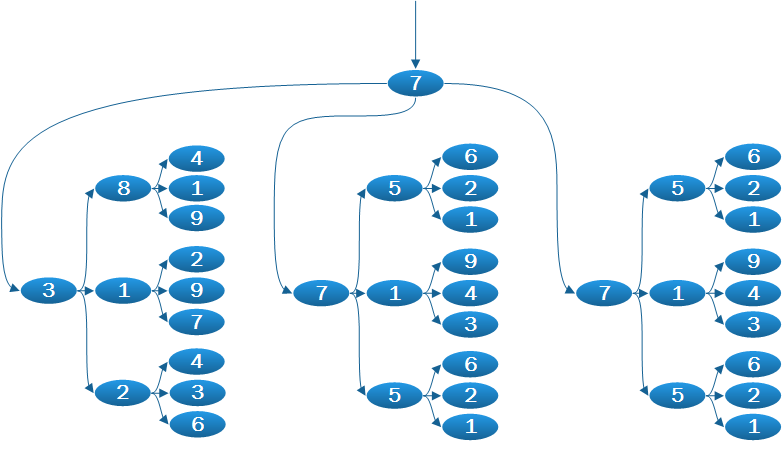
\includegraphics[width=1\textwidth]{images/wave.png}
  \caption
    [Wave propagation in Tarsier]
    {Wave propagation in Tarsier}
  \label{fig:tarsier-wave}
\end{figure}

\section{Tarsiers synchronization}
To be able to discover all the Tarsiers and to help each one of them find the others so it can send waves to them I~will use Consul \cite{consul}. Consul is designed for service discovery and makes it easy to register services and to discover them later. Each Tarsier will register itself at startup and then it will periodically check its buddies. To ensure that Consul will provide only active Tarsier instances, it has multiple types of health checks. Tarsier will have to provide some service stats.

At first I~wanted to just add some special URLs for this service stuff such as \lstinline{/health_check} and \lstinline{/metrics} but then I~realized that in the future those URLs may be needed and also those URLs don’t have to be accessible from the public network so I~designed Tarsiers with another extra interface on its own port were private data will be provided. There will be health check and metrics handler with Prometheus statistics about how many requests have been served and what commands were executed and if they were successful. I~also created a command handler where all the registered commands with their names and descriptions are provided. Because there will be plugin to simulate heavy load of memory and CPU I~add a handler that shows runtime statistics from Go. There can be seen how much memory is allocated to the Go runtime, a garbage collector statistics and much more interesting data.

\section{Tarsier plugins and their commands}

\subsection{Heavy load}
Plugin for simulating heavy load of memory and CPU
\begin{description}
  \item[Gobble RAM] will gobble as much RAM as is specified in the data. When this amount of memory is not possible to allocate it will try to resize the amount with the specified ratio and return how many bytes it finally allocated. Memory is allocated via mmap system call so the garbage collector will not free it and is filled with zeros otherwise system will not physically allocate it.
  \item[RAM stats] will show allocated mmap regions with their sizes.
  \item[Free RAM] This command will unmap allocated region. Its data is the index of the region obtained from the RAM stats command or -1 which means to free all allocated spaces.
  \item[Spin CPU] spins the CPU for the specified time. The spinning is simply done by an infinite loop with acomputation (multiply and division) with float64 numers.
\end{description}

\subsection{Faults}
\begin{description}
  \item[Deadlock] will create the specified number of goroutines that will be set to be sticky with system threads (otherwise Go runtime is allowed to move them all into single system thread, so it has no effect) and deadlock them all waiting for mutex unlock. After the defined time the handler will unlock the mutex so all goroutines will finaly end.
  \item[Segfault] will simulate segmentation fault. It uses Go unsafe package pointer to variable, which is moved out of bounds and dereferenced. The whole Tarsier will fault and it is expected that Kubernetes will start new instance.
\end{description}

\subsection{Net}
This package is here to wrap all the network commands. There are no commands for writing or reading from the network but that can be easily simulated with a dummy command to the Tarsier where waves count will be high enough.

\begin{description}
  \item[Dial] will open a new network connection to the specified address. It can open a new TCP or UDP connection and also this connection can be established directly to an IP address or to a domain name with its resolving. Those connections are set not to timeout and are not closed.
  \item[Stats] will show the network connections usage.
  \item[Close] will close the specified network connection from the Stats command. When -1 is set it closes all connections.
\end{description}

\subsection{Persistent storage}
Plugin that is working with persistent storages, typically hard disks. This plugin needs to get directory from configuration of Tarsier otherwise system temporary directory is used.

\begin{description}
  \item[Open FD] will open as many file descriptors as defined.
  \item[Read] This command will read the specified amount of bytes from defined file. Typically \lstinline{/dev/urandom} is set as a file. There is also an option how many concurrent readers are supposed to be created.
  \item[Write] will write the specified amount of bytes to opened file descriptors. There can be set how many concurrent writers are supposed to be created and each one is writing to its own file. If there is not enough file descriptors ready, new ones will be opened.
  \item[FS stats] will show usage of file descriptors, their names and sizes.
  \item[Close FD] will close the specified file descriptors from the FS stats command. When -1 is set then all file descriptors are closed and the files are deleted from the hard drive.
\end{description}

\subsection{Sleeping beauty}
Plugin for simulating requests delay.
\begin{description}
  \item[Sleep] will answer after the specified time expires.
\end{description}

\chapter{Testing the cluster}

Running applications in Kubernetes means to create some specifications for them. For testing the cluster with my Tarsier application I will need to have the Consul running at first.

I have prepared the replication controller configuration for Consul and also the service configuration for it, so it will have the same IP address regardless of which machine it is running on. The Consul will be used for a service discovery among Tarsiers. There is no need to use persistent storage for Consul, holding instances in memory is sufficient enough.

Before Tarsier pod can be created I have to register secrets for it. There will be two of them. The first secret is a SSL certificate so our service port can be run on HTTPS. The second secret is the Tarsier configuration. It is a good idea to use secrets for configuration because there can be different secrets with different configurations on the development and the production cluster and also we don’t need to rebuild the whole images just because one text file changed.

With the secrets set up, it remains to solve the persistent storage. For logs I will use the \lstinline{hostPath} volume which is a directory on the physical machine. There will be uniform policy that perhaps in \lstinline{/www/logs/} all pods will store their logs. This way it is provided that logging from the application is fast (to the local drive) and logs will remain there even when the pod dies. Also each pod should use the Kafkafeeder to feed logs to Kafka and delete them after successful upload.
 
For persistent storage plugin of Tarsier I have to use a real persistent volume. There are many applications in Seznam.cz which need a large amount of data for their start or/and which produce a large amount of data. For those data we have to choose a persistent storage where pod traveling from one machine to another will not be a problem.

I started 2 GlusterFS \cite{glusterfs} servers and created endpoints and service configuration for them. Now I can set a volume claim in the Tarsier replication controller configuration and use it without knowing the exact location of the GlusterFS and other paths.

In the Tarsier RC configuration will be more than one container. The second one will be the Kafkafeeder, which also produces logs, so it stores them to \lstinline{/www/logs/kafkafeeder} as well. Then it loads this directory and starts watching it and uploading logs to Kafka. After setting those volumes I realized that the current usage, where application creates symlink from its log directory to the \lstinline{kafkafeeder.yaml} file in the configuration directory, is no more useful. The kafkafeeder. YAML file which tells the Kafkafeeder where and which logs to upload is stored as another secret in Kubernetes and mounting this file as a volume with logs from the \lstinline{hostPath} is not possible. I solved this problem by adding another container to the pod, which is created from a simple image with a single static application. User passes the source and the target file to that application and it simply copies it. The snippet of the replication controller is as follows in listing \ref{lst:tarsier-rc}.

With those configurations prepared, the last one missing is the Tarsier service. Then I will scale the Tarsier to many instances and start sending commands to its interface.

\newpage
\begin{lstlisting}[language=yaml,caption={Snippet of replication controller configuration},label={lst:tarsier-rc}]
containers:
  - name: tarsier
    volumeMounts:
      - name: tarsier-logs
        mountPath: /www/tarsier/logs

  - name: kafkafeeder
    volumeMounts:
      - name: kf-logs
        mountPath: /www/kafkafeeder-beta/logs/

  - name: cp
    args:
      - "/src/kafkafeeder.yaml"
      - "/dst/kafkafeeder.yaml"
    volumeMounts:
      - name: tarsier-kafkafeeder
        mountPath: /src/
      - name: tarsier-logs
        mountPath: /dst/

volumes:
  - name: tarsier-logs
    hostPath: { path: /www/logs/tarsier/ }
  - name: tarsier-kafkafeeder
    secret: { secretName: tarsier-kafkafeeder }
  - name: kf-logs
    hostPath: { path: /www/logs/ }
\end{lstlisting}

\chapter{Benchmarking Python and Go application servers}

Traffic on Seznam.cz applications is high and it moves around a few thousands requests per second per one instance of an application. Python \cite{python} is used for most of our application servers, especially the Tornado framework \cite{tornado} which can handle requests asynchronously and is more lightweight \cite{flask-django-tornado} that frameworks like Django \cite{django} or Flask \cite{flask}. I~decided to benchmark such Python server and compare its performance with a server written in Go \cite{golang}. Go is a relatively young programming language, yet there are many big applications that use it. Kubernetes and Docker are both written in Go. There are also many libraries for Go, which makes it more interesting for us than Rust for example.

I~developed two simple servers which handle GET requests, generate HTML output based on a template and return the response. In Python I~used the Jinja2 \cite{jinja2} templating system, in Go I~relied on the built-in \lstinline{html/template} package. Both servers compose the output using a layout template and both render one variable in the template.

I~started those servers in Kubernetes and exposed their ports as a service. Then I~had to choose which benchmarking tool to use, so I~picked wrk \cite{wrk}.
 
Wrk is a modern HTTP benchmarking tool capable of generating a significant load when run on a single multi-core CPU. It combines a multithreaded design with scalable event notification systems such as epoll and kqueue \cite{wrk}.

Wrk allows to modify the number of client threads and the count connections opened simultaneously. I~started with 50 threads and 2000 connections opened at once. Each test was firstly start with 10 second interval for warming up the server and then repeated 3 times with 2 minute length.

I~started both servers in Kubernetes and allowed them to use only one CPU core. Then I~was adding cores to the servers and ran this test again and again.

For the testing I~used a bare-metal server with the Debian Jessie operating system installed. The hardware configuration of this machine was 24 Intel Xeon processors at 2.27 GHz and 32 GB of RAM. Both servers were running in Docker on one machine and I~used another one to run the benchmarks one after another.

The request rate per second is shown in the graph \ref{fig:benchmark-requests} and the average latency in the graph \ref{fig:benchmark-latency}.

From the graphs we can see that the Go application server is far much faster and is scaling linearly with the CPU count. The top boundary of the scaling was about 33 000 requests per second and was most likely held back by the network limits in the developer VLAN where my machines were placed. Python scales well in the beginning but with an increasing CPU count it starts to scale more slowly. Even with all of the 24 CPUs involved it didn’t achieved the performance of the Go server and that is a good reason to start writing our application servers in the Go language.

\begin{figure}[htb]\centering
  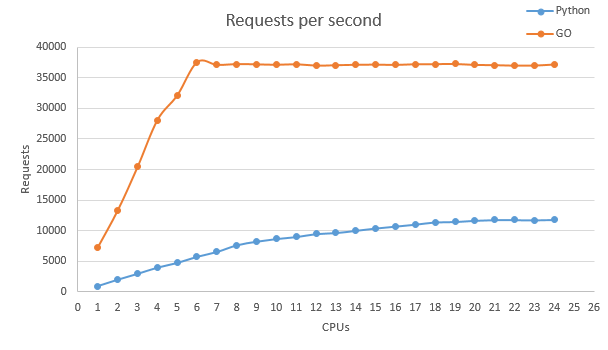
\includegraphics[width=1\textwidth]{images/benchmark-requests.png}
  \caption
    {Benchmarking Python and Go -- Requests per second}
  \label{fig:benchmark-requests}
\end{figure}
                                                  
\begin{figure}[htb]\centering
  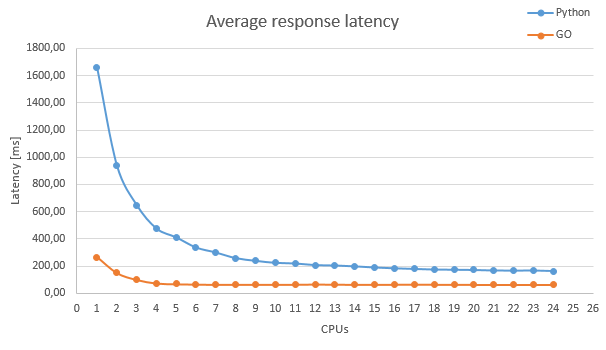
\includegraphics[width=1\textwidth]{images/benchmark-latency.png}
  \caption
    {Benchmarking Python and Go -- Average response latency}
  \label{fig:benchmark-latency}
\end{figure}
                                                  
\begin{figure}[htb]\centering
  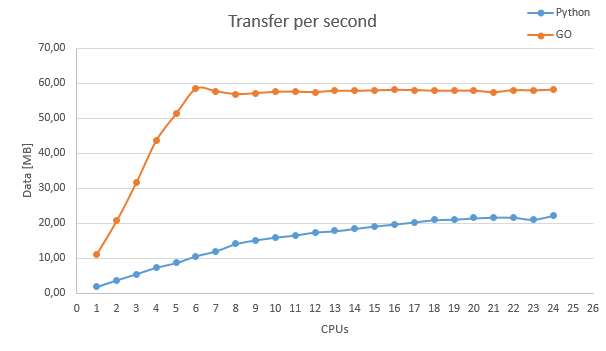
\includegraphics[width=1\textwidth]{images/benchmark-transfer.png}
  \caption
    {Benchmarking Python and Go -- Transfer per second}
  \label{fig:benchmark-transfer}
\end{figure}
\chapter{Benefits for Seznam.cz}

In the chapter ``\nameref{chapter:seznam-nowadays}" I~described how the developers are working today, what do they have to do and how the administrators are managing the machines. What is the motivation to switch to a solution based on Docker and Kubernetes and how to spread this new idea around? Obviously, apart from all the problems we identified before, there also have to be certain key benefits for both the developers and the administrators, otherwise it wouldn’t make sense to use it.

The biggest benefit I~see as a developer is that when an environment is created and deployed in the production environment, the developers can still access it easily. That is something I~miss a lot nowadays. The administrators prepare the virtual machine in the production using their Salt \cite{salt} prescriptions and then install packages from the developers. The developers are building and testing packages on their own virtual machines they create. There can be differences in many things from the network settings to different source list and different versions of libraries. It is also difficult to maintain virtual machines for building and testing for developers who could spend that time coding instead.

Docker solves those problems. Developer knows which packages in which version he needs, so he creates a Dockerfile with it. His image will be built from a base image provided by administrators where all the necessary settings are done and the same image will be used both in the production and in the testing environment. 

Docker also solves problems with library versions. Typical example may be one virtual machine where one service is running which consists of many packages and many smaller micro services. Each of this micro service is maintained by a different developer from the same team. When one of them changes somethings and wants to upgrade his micro service but he depends on a newer library, all other micro services will have to be updated as well. But with Docker, he just pushes the new image that will be updated in pod and no one else intervention is needed.

For the administrators the deployment will be easier as well. The developer defines the whole environment in a single image, so they just have to start it. The problem will be with debugging issues that occur in operation, because nowadays they can connect to any server and use debug tools they want and know. With Docker images in Kubernetes they first have to find the right container so they can attach to it, but if that image was created from scratch, no tools are provided there. In the beginning of our Kubernetes experience we should probably create all images from a base Debian image tailored to our needs so the administrators can use the same tools that they are used to. Then in the future we can move to more lightweight solutions.

Another inconvenience that the Kubernetes solution will solve is the secrets and configuration distribution. When the product manager wants a configuration change, for example setting a lower bound of a delivery score, the developer currently has to repack the application and issue a request ticket. The administrator then stops traffic to one server, installs the new version and restarts the application. After confirming that everything is alright, he can move on with the rest of the servers. With Kubernetes the developer will simply update the configuration, generate secret, push it to Git and send a merge request to the administrator. When the administrator accepts it, he updates the secret in the Kubernetes cluster and starts rolling update (or just sends signal to container, if the application supports configuration reload when running). Also SSL certificates can be stored in the Kubernetes cluster for development and production.

With Kubernetes the developers don’t need to maintain virtual machines for testing anymore. The administrators start two (or even more) instances of the Kubernetes cluster in the production and in the testing environment. The same pods, secrets and other resources will be deployed to those clusters.

Economic benefit is also that fewer servers is needed because they will be used more effectively. We can scale applications fast and more adaptively. Traffic will be monitored and examined and there surely be services that have minimal traffic in night so their number can be reduced dynamically.

The idea for the future not so far away is to use the same cluster which means the same machines in production delivery (services such as homepage and others) and for internal tasks like counting signals of webpages, machine learning of our algorithms and so more. If we group all machines in the data centre to one cluster and define proper policies for pod preference and priority, we can use the whole potential of this cluster at night and still have sufficient availability for users who access our services at the same time. This is the future goal were we are heading for.


\setsecnumdepth{part}
\chapter{Conclusion}

The goal of the suitability analysis of Kubernetes for Seznam.cz was to become familiar with the basics such as using Docker and virtualization in general. That’s why the beginning of this thesis is dedicated to the theory about Docker containers and using Kubernetes for orchestrating them. 

The next step was to employ those information in Seznam.cz’s specific environment. I~mapped and examined the current situation of application development and deployment at Seznam.cz and was wondering about how to upgrade it and how to make use of container virtualization there. I~focused on possible problems such as creating the Docker registry, how to deal with the security and contents of images, how to log and where to store logs for further analysis and I~also had to have in mind that containers are able to move between machines but logs have to be processed correctly. I~had to propose how to monitor the applications in the containers and also the containers themselves. And I~had to find out how to deploy the static content of the webpages using load balancers.

I~successfully dealt with all of those issues and after consulting with our security administrators I~suggested how to secure and monitor what is in the images that we are running. I~suggested the architecture of the Docker registry we have to build. This architecture achieved high availability thanks to the Swift storage on which the Docker registry will be running in each data centre. I~explored different network management solutions that are possible to use in Kubernetes and chose to start the cluster with the flannel. The flannel has a significant overhead compared to other possibilities but it is sufficient for the purposes of my thesis.

It is important to know how the new Kubernetes cluster is behaving under heavy load and in other specific situations such as deadlocked applications, too many open files or network connections, so I~developed an application for testing such cluster. This application uses secrets with SSL certificates, secrets with configuration and produces logs. It also uses a persistent storage, for which I~utilized GlusterFS servers. The application provides Prometheus metrics on its service interface. Moreover I~created another application that watches a specified directory and sends logs to kafka for further processing. I~had to resolve many problems with reliability and performance and I~handled them successfully and implemented the Kafkafeeder application which will be present in each pod for uploading the logs.

In the end I~focused on better repeatability of the cluster creation procedure and I~wrote scripts that simplify installing it again later or adding new nodes to the existing cluster. I~wrote the Kubernetes configurations for my applications, creating services, secrets and other prescriptions used in Kubernetes.

During my work on this thesis I~found answers for many generic issues associated with starting the Kubernetes cluster while only a few of them were specific for Seznam.cz, so I~decided to open source all my code and images I~created. Those applications, images and the Kubernetes configurations can be used as examples for further development and can help others as well.


\bibliographystyle{inc/iso690}
\bibliography{bibliography}

\setsecnumdepth{all}
\appendix

\chapter{Acronyms}
\begin{description}
	\item[PaaS] Platform as a service    
	\item[RC] Replication Controller 
	\item[IP] Internet Protocol 
	\item[API] Application Programming Interface
	\item[REST] Representational State Transfer
	\item[CPU] Central processing unit
	\item[HTML] HyperText Markup Language 
	\item[CSS] Cascading Style Sheets
	\item[eth] Ethernet network interface
	\item[veth] Virtual Ethernet device 
	\item[NAT] Network Address Translation  
	\item[UDP] User Datagram Protocol   
	\item[TCP] Transmission Control Protocol 
	\item[TUN] Network tunnel
	\item[VM] Virtual machine
	\item[SDN] Software-defined networking 
	\item[GET] HTTP method
  \item[POST] HTTP method           
  \item[HTTP] Hypertext Transfer Protocol
  \item[HTTPS] Hypertext Transfer Protocol Secure  
	\item[RAM] Random-access memory
	\item[VLAN] Virtual LAN
  \item[LAN] Local area network
  \item[HDFS] Hadoop Distributed File System
  \item[stdin] Standard input I/O connection 
  \item[stdout] Standard output I/O connection 
  \item[stderr] Standard error I/O connection
  \item[I/O] input/output  
  \item[JVM] Java virtual machine
  \item[SIGTERM] Generic signal used to cause program termination
  \item[SIGCHLD] When a child process stops or terminates, SIGCHLD is sent to the parent process 
  \item[npm] Package manager for JavaScript 
  \item[GCC] GNU Compiler Collection
  \item[GNU] GNU's Not Unix! 
  \item[PIP] Pip Installs Packages, Pip Installs Python
  \item[CDN] Content delivery network
  \item[YAML] YAML Ain't Markup Language
  \item[JSON] JavaScript Object Notation 
  \item[FD] Ffile descriptor
  \item[SSL] Secure Sockets Layer  
  \item[URL] Uniform Resource Locator 
\end{description}

\chapter{Contents of enclosed CD}
\begin{figure}
	\dirtree{%
		.1 readme.txt\DTcomment{the file with CD contents description}.
		.1 src\DTcomment{the directory of source codes}.    
      .2 go-kafkalog\DTcomment{Apache Kafka log format implementation in Go}.  
      .2 go-ultimate-server\DTcomment{Go server for benchmarking}.  
      .2 heka\DTcomment{Some Heka adjustment for greater reliability }.  
      .2 heka-kafkalog\DTcomment{Splitter and Decored plugins}.
      .2 kafkafeeder\DTcomment{Application that transfers logs to Kafka}.  
      .2 kafkalog-logrus\DTcomment{Kafkalog hook to logrus}.  
      .2 kubernetes-testing\DTcomment{Support scripts for testing Kubernetes}.  
      .2 python-ultimate-server\DTcomment{Python server for benchmarking}.  
      .2 tarsier\DTcomment{Application fer testing Kubernetes cluster}.
		.1 text\DTcomment{the thesis text directory}.
  	  .2 appendix\DTcomment{cd contents file and acronyms}.
  	  .2 chapters\DTcomment{files of each chapter}.
  	  .2 images\DTcomment{all used images}.
  	  .2 inc\DTcomment{includes such as assignment, logo, class file, \ldots}.
  	  .2 bibliography.bib\DTcomment{bibliography file}.
  	  .2 sejvlond\_masters\_thesis.tex\DTcomment{main tex file}.
      .2 sejvlond\_masters\_thesis.pdf\DTcomment{final PDF}.      
	}
\end{figure}


\end{document}